\documentclass[11pt]{article}
\usepackage[a4paper,margin=26mm]{geometry}
\usepackage[T1]{fontenc}
\usepackage{lmodern}
\usepackage{amsmath,amssymb,amsthm}
\usepackage{microtype}
\usepackage{array}
\usepackage{tikz}
\usepackage{xurl}
\usepackage{hyperref}
\hypersetup{colorlinks=true,linkcolor=blue,urlcolor=blue,citecolor=blue,
 pdftitle={Multisets of bars that do not tile a 2 x n rectangle: the optimal growth order},
 pdfauthor={Horace Dong}}
\newtheorem{theorem}{Theorem}
\newtheorem{lemma}{Lemma}
\newtheorem{proposition}{Proposition}
\newtheorem{corollary}{Corollary}
\theoremstyle{definition}
\newtheorem{definition}{Definition}
\theoremstyle{remark}
\newtheorem{remark}{Remark}
\newcommand{\repoversion}{1.25.0}
\setlength{\emergencystretch}{1.5em}
\newcommand{\area}{\operatorname{area}}

\title{Multisets of bars that do not tile a $2\times n$ rectangle:\\ the optimal growth order}
\author{Horace Dong\\ \small Independent researcher\\
\small\texttt{maxwelldhx@gmail.com}\\
\small ORCID: \href{https://orcid.org/0009-0002-7554-7548}{0009-0002-7554-7548}}
\date{22 November 2026}
\begin{document}
\maketitle

\begin{abstract}
For $k\ge1$ let $D_k(n)$ be the number of multisets of bars $1\times\ell$
($1\le\ell\le k$) of total area $2n$ that cannot be arranged to tile the
$2\times n$ rectangle; in the notation of Gajdzica, Visser and Zakarczemny,
$D_k(n)=|p_{k,1}(2,n)-p_k(2n)|$. In their Remark~5.11 they observe, from
conjectured formulas for $4\le k\le 8$, that this difference is $O(1)$ for
$k\le5$, $O(n)$ for $k=6,7$ and $O(n^2)$ for $k=8$, and they ask for a tight
upper bound for all $k$. We show that $D_k(n)=0$ for $k\le2$ and that for
every $k\ge3$ there is a constant $C_k$ with $D_k(n)\le C_k(n+1)^{e}$ for all
$n\ge1$, where $e=\max(0,\lfloor k/2\rfloor-2)$. This exponent cannot be
lowered: $D_k(n)\ge c_k(n+1)^e$ with $c_k>0$ along arbitrarily large $n$, namely
at every sufficiently large odd $n$ when $k\ge6$ and at every $n\equiv2\pmod 3$
when $3\le k\le5$. In particular the three observations of Remark~5.11 hold
unconditionally and are sharp. The proof uses a two-row criterion for
tileability, a bounded Bézout argument, and families of bars of even length.
The result, together with the equivalence between the geometric definition
of a tiling and the two-row criterion, is formally verified in Lean~4. The
proofs were found and formalized by AI agents working under the author's
direction; their role is described at the end of the paper.
\end{abstract}

\section{Introduction}

Gajdzica, Visser and Zakarczemny~\cite{gvz} count partitions of a rectangle
into rectangular blocks. Following their Definition~1.1, a rectangle is a set
$[a,b]\times[c,d]\subset\mathbb R^2$ with $a<b$, $c<d$. A \emph{partition} of
$R=[0,m]\times[0,n]$ (Definition~1.2) is a multiset of rectangles with
positive integer side lengths, a block $k\times l$ being indistinguishable from
a block $l\times k$, such that the blocks ``can be arranged in such a way that
they cover exactly the area of the rectangle $R$ and their interiors do not
intersect''; two partitions are the same if they are equal as multisets. The
arrangement itself is not counted, and positions are real numbers.

In Section~5 of~\cite{gvz}, $p_{k,l}(2,n)$ is the number of partitions of the
$2\times n$ rectangle in which only blocks $1\times i$ with $1\le i\le k$ and
$2\times j$ with $2\le j\le l$ are allowed. For $l=1$ only the bars
$1\times1,\dots,1\times k$ remain; the bar $1\times2$ may stand vertically (as
a $2\times1$ block), and longer bars cannot, since they do not fit across the
short side. Every partition counted by $p_{k,1}(2,n)$ is a multiset of bars of
total area $2n$, that is, a partition of the integer $2n$ into parts at most
$k$; the number of these is the classical $p_k(2n)$ (equivalently, by
conjugation, the number of partitions of $2n$ into at most $k$ parts). So
\[
D_k(n):=p_k(2n)-p_{k,1}(2,n)=|p_{k,1}(2,n)-p_k(2n)|\ \ge 0
\]
is the number of multisets of bars of lengths at most $k$ and total area $2n$
that do \emph{not} tile the $2\times n$ rectangle. For instance, a bar
$1\times3$ and a unit square have area $4$ but do not tile the $2\times2$
square, so $D_3(2)\ge1$.

For $4\le k\le8$ the authors computed conjectured quasi-polynomial formulas for
$p_{k,1}(2,n)$ (their Table~2), and wrote in Remark~5.11:

\begin{quote}
From Table 2, we note that we actually have $|p_{k,1}(2,n)-p_k(2n)|=O(1)$
for $k\le5$, $|p_{k,1}(2,n)-p_k(2n)|=O(n)$ for $k\in\{6,7\}$, and
$|p_{k,1}(2,n)-p_k(2n)|=O(n^2)$ for $k=8$. In general, it seems an
interesting problem to compute a tight upper bound for
$|p_{k,1}(2,n)-p_k(2n)|$ for all $k$.
\end{quote}

\noindent The quotation follows the journal version~\cite{gvz}, where
Remark~5.11 begins on page~22 of the article PDF and the question is on
page~24 (Table~2 is on page~23); in arXiv:2509.20495v2 the same remark, with
the same number and the same question, is on page~17. Section~5 has the same
numbering in both versions. For $k\le3$ the observation follows from the proved formulas of
Proposition~5.5 of~\cite{gvz} together with the classical formulas for
$p_k(2n)$; for $4\le k\le8$ it rests on
the conjectured formulas of Table~2.

We answer the question in the sense of the optimal polynomial order, which is
the sense of the three observations above. Throughout,
\[
e_k=\max\bigl(0,\lfloor k/2\rfloor-2\bigr),
\]
so $e_k=0$ for $k\le5$, $e_6=e_7=1$, $e_8=e_9=2$, and in general $e_k$ grows
like $k/2$.

\begin{theorem}\label{thm:main}
\begin{enumerate}
\item[(a)] If $k\in\{1,2\}$, then $D_k(n)=0$ for every $n\ge1$.
\item[(b)] For every $k\ge3$ there is a constant $C>0$ such that
$D_k(n)\le C\,(n+1)^{e_k}$ for every $n\ge1$.
\item[(c)] For every $k\ge3$ there is a constant $C>0$ such that for every
$N$ there is $n\ge N$ with $(n+1)^{e_k}\le C\,D_k(n)$.
\item[(d)] For every $k\ge6$ there are constants $C>0$ and $N$ such that
$(n+1)^{e_k}\le C\,D_k(n)$ for every odd $n\ge N$.
\end{enumerate}
\end{theorem}

\noindent The constants depend on $k$. Part~(c) says that the bound in~(b)
is not $o(n^{e_k})$; for $3\le k\le5$, where $e_k=0$, it says that $D_k(n)\ge1$
for infinitely many $n$, so the bound $O(1)$ cannot be improved to ``eventually
zero''. The proof gives more for $3\le k\le5$: $D_k(n)\ge1$ for every
$n\equiv2\pmod3$ (Proposition~\ref{prop:lower35}). Theorem~\ref{thm:main} is
the statement verified in Lean (Section~\ref{sec:lean}). The constant in~(b)
comes from a finite choice of Bézout coefficients and is not explicit; in~(d)
one can take $C=(2D)^{e_k}$ and $N=D$ with $D=2k^2+4$. We make no claim about
leading constants.

\begin{corollary}\label{cor:remark}
The three observations of Remark~5.11 of~\cite{gvz} hold for all $n\ge1$,
without the conjectured formulas of Table~2, and each is sharp:
$D_k(n)=O(1)$ for $k\le5$, with $D_k(n)=0$ for $k\le2$ and $D_k(n)\ge1$ for
infinitely many $n$ (indeed for all $n\equiv2\pmod 3$) when $3\le k\le5$;
$D_k(n)=O(n)$ for $k=6,7$ and $D_k(n)=O(n^2)$ for $k=8$, and in these cases
$D_k(n)\ge c_k n^{e_k}$ for every large odd $n$, with $c_k>0$.
\end{corollary}

\noindent The corollary is Theorem~\ref{thm:main} specialized to $k\le8$; the
specialization is immediate and is not a separate Lean declaration, and the
congruence $n\equiv2\pmod3$ comes from a lemma inside the Lean proof
(Section~\ref{sec:lean}).

\begin{remark}\label{rem:subseq}
The matching lower bound is claimed only along subsequences: every large odd
$n$ for $k\ge6$, and $n\equiv2\pmod 3$ for $3\le k\le5$. Nothing is claimed
about $\liminf D_k(n)/n^{e_k}$, and on some even widths the defect is much
smaller. For example $D_6(36)=2$, while $D_6(35)=36$ and $D_6(37)=27$. These
values, and those of Table~\ref{tab:small}, were computed with the two-row
criterion of Proposition~\ref{prop:criterion} by short programs; they are not
part of the Lean files.
\end{remark}

\begin{table}[ht]
\centering\small
\begin{tabular}{c|cccccccccc}
$k\backslash n$ & 1&2&3&4&5&6&7&8&9&10\\ \hline
3 &0&1&0&0&1&0&0&1&0&0\\
4 &0&2&2&0&2&2&2&2&1&2\\
5 &0&2&3&3&2&3&6&5&4&4\\
6 &0&2&4&5&7&3&8&11&11&10\\
7 &0&2&4&6&10&10&8&14&19&19\\
8 &0&2&4&7&12&15&19&14&23&31
\end{tabular}
\caption{Small values of $D_k(n)$ (computed, not in Lean). For $k\le8$ and
$n\le10$ these were obtained both by enumerating tilings of the $2\times n$
grid and with the criterion of Proposition~\ref{prop:criterion}, which agreed
on all $4308$ count vectors with $1\le k\le8$ and $1\le n\le10$.}
\label{tab:small}
\end{table}

\subsection*{Prior work}
Gajdzica, Visser and Zakarczemny~\cite{gvz} give explicit formulas for
$p_{k,l}(2,n)$ with $k,l\le3$ (Proposition~5.5), the leading-term estimate
$p_{k,1}(2,n)=(2n)^{k-1}/(k!(k-1)!)+O(n^{k-2})$ (Proposition~5.8), and the
conjectured formulas of Table~2. Shaikh's preprint~\cite{shaikh} gives a proof of the neighbouring
Conjecture~5.10 (eventual quasi-polynomiality and the denominator of the
generating function); he does not address Remark~5.11. Three further 2026
papers on rectangle partitions treat different questions: Gajdzica and
Zakarczemny~\cite{gz1} determine the asymptotics of $\log p(n,n)$ and
$\log p(3,n)$; Gajdzica and Zakarczemny~\cite{gz2} determine
$\log p(m,n)$ for fixed $m$; and the November preprint of
Shukla~\cite{shukla} approximates the number $r(n)$ of multisets of arbitrary
integer-sided rectangles tiling the $2\times n$ rectangle by cubic partition
numbers, with an error term of lower exponential order (according to its abstract). None of these restricts the length of the bars or treats the
difference in Remark~5.11. As far as we know, the question of Remark~5.11 has
not been answered elsewhere; the searches are described in the final section.

\section{A two-row criterion}\label{sec:criterion}

We encode a multiset of bars by its \emph{count vector}
$m=(m_1,\dots,m_k)\in\mathbb Z_{\ge0}^k$, where $m_\ell$ is the number of bars
$1\times\ell$, and write $\area(m)=\sum_\ell \ell\,m_\ell$. Inequalities and sums of count vectors are taken coordinatewise.
As in~\cite{gvz} we take $R=[0,2]\times[0,n]$; the first coordinate runs across
the short side. A bar of length $\ell$ placed at $(\alpha,\beta)\in\mathbb R^2$
occupies $[\alpha,\alpha+\ell]\times[\beta,\beta+1]$ if it is placed across
the strip and $[\alpha,\alpha+1]\times[\beta,\beta+\ell]$ if it is placed
along it. We say that $m$ \emph{tiles} $R$ if every bar of the multiset can be
given a position and a direction so that the union of the closed bars is $R$
and distinct bars have disjoint interiors. This is Definition~1.2 of~\cite{gvz}
for bars.

\begin{definition}
Let $\area(m)=2n$. A \emph{row split} of $m$ is a decomposition $m=a+b+v$ into
count vectors with $v$ supported on the length $2$ (that is, $v_\ell=0$ for
$\ell\ne2$) such that
\[
\area(a)+v_2=n\qquad\text{and}\qquad\area(b)+v_2=n .
\]
\end{definition}

\noindent Here $v$ counts dominoes placed across the strip, and $a$ and $b$
are the bars in the two rows (Figure~\ref{fig:split}).

\begin{figure}[ht]
\centering
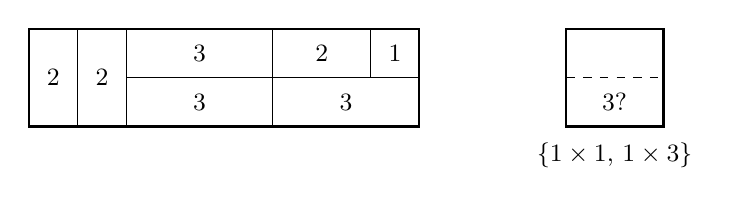
\begin{tikzpicture}[scale=0.62]
\draw[thick] (0,0) rectangle (8,2);
\foreach \x in {0,1} \draw (\x,0) rectangle (\x+1,2);
\draw (2,0) rectangle (5,1); \draw (5,0) rectangle (8,1);
\draw (2,1) rectangle (5,2); \draw (5,1) rectangle (7,2); \draw (7,1) rectangle (8,2);
\node at (0.5,1) {\small 2}; \node at (1.5,1) {\small 2};
\node at (3.5,0.5) {\small 3}; \node at (6.5,0.5) {\small 3};
\node at (3.5,1.5) {\small 3}; \node at (6,1.5) {\small 2}; \node at (7.5,1.5) {\small 1};
\begin{scope}[xshift=11cm]
\draw[thick] (0,0) rectangle (2,2);
\draw[dashed] (0,0) rectangle (2,1);
\node at (1,0.5) {\small 3?};
\node at (1,-0.6) {\small$\{1\times1,\,1\times3\}$};
\end{scope}
\end{tikzpicture}
\caption{Left: a row split of the multiset with one bar of length $1$, three
of length $2$ and three of length $3$ in the $2\times8$ rectangle (long side
drawn horizontally): $v_2=2$ dominoes across the strip and two rows of length
$6$. Right: a bar $1\times3$ and a unit square have area $4$ but do not fit
in the $2\times2$ square.}
\label{fig:split}
\end{figure}

\begin{proposition}\label{prop:criterion}
Let $n\ge1$ and $\area(m)=2n$. Then $m$ tiles $[0,2]\times[0,n]$ if and only
if $m$ has a row split.
\end{proposition}

\begin{proof}
Suppose $m=a+b+v$ is a row split and put $F=v_2$. Place the $F$ dominoes
across the strip at $[0,2]\times[j,j+1]$, $0\le j<F$. Place the bars of $a$
along the strip end to end in the row $[0,1]\times[F,n]$, starting at $F$, and
those of $b$ in the row $[1,2]\times[F,n]$; since $\area(a)=\area(b)=n-F$,
each row is filled exactly. The closed bars cover $R$, and distinct bars have
disjoint interiors. If a row is empty, then $F=n$ and the dominoes alone cover
$R$; here $n\ge1$ is used, since for $n=0$ the empty multiset does not cover
the segment $[0,2]\times\{0\}$.

Conversely, fix a tiling, and write each placed bar as
$[\alpha,\alpha+h]\times[\beta,\beta+w]$, where $(h,w)=(\ell,1)$ or $(1,\ell)$,
so that $h\ge1$. Since the bar lies in $R$, $0\le\alpha$ and $\alpha+h\le2$;
in particular only bars of length at most $2$ can lie across the strip. Let
$S$ be the set of bars with $\alpha=0$, the bars touching the side
$\{0\}\times[0,n]$. For $y\in[0,n]$ the point $(0,y)$ lies in some bar, which
must have $\alpha=0$; so the intervals $[\beta,\beta+w]$ of the bars in $S$
cover $[0,n]$. Their interiors are pairwise disjoint: if two of them contained
a common $y$, the point $(\frac12,y)$ would lie in the interiors of two bars,
because $0<\frac12<1\le h$. Comparing Lebesgue measures gives
$\sum_{S}w=n$. Let $v$ count the dominoes in $S$ placed across the strip (for
them $w=1$), let $b$ count the other bars in $S$ (for them $w$ is the length
of the bar, a unit square having $w=1$), and let $a$ count all remaining bars.
Then $\area(b)+v_2=n$, and
$\area(a)=\area(m)-\area(b)-2v_2=2n-(n-v_2)-2v_2=n-v_2$. So
$m=a+b+v$ is a row split. No integrality of the positions is assumed.
\end{proof}

\noindent In Lean the two directions are \texttt{rowSplit\_\allowbreak of\_\allowbreak tiles}
and \texttt{tiles\_\allowbreak of\_\allowbreak rowSplit}, and the equivalence is
\texttt{tiles\_\allowbreak iff\_\allowbreak rowSplit}. Thus $D_k(n)$ is the number
of count vectors of area $2n$ without a row split.

\section{\texorpdfstring{The cases $k\le2$ and the upper bound}{The cases k <= 2 and the upper bound}}\label{sec:upper}

\begin{proof}[Proof of Theorem~\ref{thm:main}(a)]
For $k=1$ take $a=b=(n)$ and $v=0$. For $k=2$ we have $m_1=2n-2m_2$; take
$v_2=m_2$ and put $n-m_2$ unit squares in each row.
\end{proof}

Fix $k\ge3$ and put $K=1+2+\dots+k$. For a finite set $J$ of positive
integers let $\gcd(J)$ be its greatest common divisor, with $\gcd(\varnothing)=0$.

\begin{lemma}[bounded Bézout]\label{lem:bezout}
There is a constant $B=B_k$ with the following property. For every
$J\subseteq\{1,\dots,k\}$ and every integer $h$ with $0\le h\le K$ and
$\gcd(J)\mid h$ there are integers $c_1,\dots,c_k$ with $c_\ell=0$ for
$\ell\notin J$, $|c_\ell|\le B$ for all $\ell$, and $\sum_\ell \ell\,c_\ell=h$.
\end{lemma}

\begin{proof}
By induction on $J$, using the two-term Bézout identity, $\gcd(J)$ is an
integer combination of the elements of $J$; multiply by $h/\gcd(J)$ (for
$J=\varnothing$ only $h=0$ occurs). There are finitely many pairs $(J,h)$;
let $B$ be the largest absolute value of a chosen coefficient.
\end{proof}

\begin{lemma}[half split]\label{lem:half}
If $\area(m)=2n$, let $\lfloor m/2\rfloor$ denote the vector with entries
$\lfloor m_\ell/2\rfloor$. Then $\area(\lfloor m/2\rfloor)+h=n$ for some
integer $0\le h\le K$.
\end{lemma}

\begin{proof}
$2\area(\lfloor m/2\rfloor)=2n-\sum_{m_\ell\ \mathrm{odd}}\ell$, so
$h=\frac12\sum_{m_\ell\ \mathrm{odd}}\ell$ lies in $[0,K]$.
\end{proof}

Let $T=2B+4$ and, for a count vector $m$, let $J(m)=\{\ell: m_\ell\ge T\}$ be
the set of \emph{heavy} lengths.

\begin{lemma}[balancing]\label{lem:balance}
Let $\area(m)=2n$, and suppose that $m$ has no row split and that $J=J(m)$ is
nonempty. Then either $\gcd(J)\ge3$, or $\gcd(J)=2$ and $2\notin J$.
\end{lemma}

\begin{proof}
Suppose instead that $\gcd(J)=1$, or that $\gcd(J)=2$ and $2\in J$. Let $h$
be as in Lemma~\ref{lem:half}. In the first case put $r=0$; in the second put
$r=h\bmod 2\in\{0,1\}$, which is allowed because $m_2\ge T\ge1$. In both cases
$\gcd(J)\mid h-r$ and $0\le h-r\le K$, so Lemma~\ref{lem:bezout} gives
coefficients $c$ supported on $J$ with $\sum_\ell\ell c_\ell=h-r$ and
$|c_\ell|\le B$. Let $v$ be $r$ dominoes ($v_2=r$), let
$a_\ell=\lfloor m_\ell/2\rfloor+c_\ell$, and let $b=m-a-v$. For $\ell\notin J$
we have $c_\ell=0$ and $v_\ell=0$. For $\ell\in J$ we have $m_\ell\ge2B+4$,
hence $a_\ell\ge0$ and $a_\ell+v_\ell\le m_\ell/2+B+1\le m_\ell$. So
$a,b,v\ge0$, and
\[
\area(a)+v_2=\area(\lfloor m/2\rfloor)+(h-r)+r=n,\qquad
\area(b)+v_2=2n-\area(a)-2v_2+v_2=n .
\]
This is a row split, a contradiction.
\end{proof}

\begin{lemma}\label{lem:sparse}
Let $k\ge3$ and let $J\subseteq\{1,\dots,k\}$ be nonempty with $\gcd(J)\ge3$,
or with $\gcd(J)=2$ and $2\notin J$. Then $|J|\le e_k+1$.
\end{lemma}

\begin{proof}
In the first case $J$ consists of multiples of some $g\ge3$, so
$|J|\le\lfloor k/3\rfloor$; in the second $J\subseteq\{4,6,\dots,2\lfloor
k/2\rfloor\}$, so $|J|\le\lfloor k/2\rfloor-1$. Both numbers are at most
$\max(1,\lfloor k/2\rfloor-1)=e_k+1$ for $k\ge3$.
\end{proof}

\begin{lemma}[counting]\label{lem:count}
Let $n\ge1$. If every count vector $m$ of area $2n$ without a row split has
$|J(m)|\le e+1$, then $D_k(n)\le 2^k(T+1)^k(2n+1)^{e}$.
\end{lemma}

\begin{proof}
Encode such an $m$ by the set $J(m)$, the truncated entries
$\min(m_\ell,T)$, and the entries $m_\ell$ for $\ell\in J(m)$ other than a
fixed pivot element of $J(m)$; there are at most $e$ of the latter, each in
$[0,2n]$ because $m_\ell\le\area(m)$. The entries outside $J(m)$ are below $T$
and are recovered from the truncation, and the pivot entry is recovered from
$\area(m)=2n$. So the code is injective, and there are at most
$2^k(T+1)^k(2n+1)^e$ codes.
\end{proof}

\begin{proof}[Proof of Theorem~\ref{thm:main}(b)]
By Proposition~\ref{prop:criterion}, $D_k(n)$ counts the vectors of area $2n$
without a row split. For such a vector, either $J(m)=\varnothing$ or, by
Lemmas~\ref{lem:balance} and~\ref{lem:sparse}, $|J(m)|\le e_k+1$. By
Lemma~\ref{lem:count}, $D_k(n)\le 2^k(T+1)^k(2n+1)^{e_k}\le
2^k(T+1)^k2^{e_k}(n+1)^{e_k}$.
\end{proof}

\section{Lower bounds}\label{sec:lower}

\begin{proposition}\label{prop:lower35}
Let $k\ge3$ and $b\ge0$. The vector with one unit square and $2b+1$ bars of
length $3$ has area $2(3b+2)$ and does not tile the $2\times(3b+2)$
rectangle. Hence $D_k(n)\ge1$ for every $n\equiv2\pmod 3$.
\end{proposition}

\begin{proof}
There are no bars of length $2$, so a row split has $v=0$, and one row holds
$a_1\le1$ unit squares and $a_3$ bars of length $3$ with $a_1+3a_3=3b+2$. This
forces $a_1\equiv2\pmod3$, which is impossible.
\end{proof}

\noindent For $3\le k\le5$ this gives Theorem~\ref{thm:main}(c), since
$e_k=0$. For $k\ge6$ we use bars of even length at least~$4$.

\begin{lemma}\label{lem:even}
If all bars of $m$ have even length at least $4$ and $n$ is odd, then $m$ does
not tile the $2\times n$ rectangle.
\end{lemma}

\begin{proof}
There are no bars of length $2$, so $v=0$ in a row split, and a row of length
$n$ would be a sum of even lengths.
\end{proof}

\begin{proposition}\label{prop:lower6}
Let $k\ge6$, $r=\lfloor k/2\rfloor$, $e=e_k=r-2$, $D=2k^2+4$, and let $n\ge D$
be odd. Then $(n+1)^{e}\le(2D)^{e}D_k(n)$.
\end{proposition}

\begin{proof}
Let $M=\lfloor n/D\rfloor\ge1$. For each $x=(x_3,\dots,x_r)\in\{0,\dots,M-1\}^{e}$
let $m(x)$ consist of $2x_j$ bars of length $2j$ for $3\le j\le r$, one further
bar of length $6$, and
\[
m_4=\tfrac{n-3}{2}-w(x),\qquad w(x)=\sum_{j=3}^r j\,x_j ,
\]
bars of length $4$. Since $w(x)\le k^2M\le k^2n/D<(n-3)/2$, this is
nonnegative, and
$\area(m(x))=4m_4+6+\sum_j 2j\cdot 2x_j=2(n-3)-4w(x)+6+4w(x)=2n$. The bars
of $m(x)$ have even length at least~$4$, so by Lemma~\ref{lem:even} no $m(x)$
tiles. The map $x\mapsto m(x)$ is injective: $x_j$ is half the number of bars
of length $2j$, after removing the extra bar when $j=3$. Hence
$D_k(n)\ge M^{e}$. Finally $n+1\le 2DM$ because $n\ge D$, so
$(n+1)^e\le(2D)^eM^e\le(2D)^eD_k(n)$.
\end{proof}

\begin{proof}[Proof of Theorem~\ref{thm:main}(c) and~(d)]
Part~(d) is Proposition~\ref{prop:lower6}. For~(c), if $k\ge6$ take the odd
widths of~(d); if $3\le k\le5$, then $e_k=0$ and Proposition~\ref{prop:lower35}
gives $1\le D_k(3N+2)$ for every $N$.
\end{proof}

{\sloppy
\section{Formal verification}\label{sec:lean}

Theorem~\ref{thm:main} is formally verified in Lean~4 (version 4.34.1) with
Mathlib~\cite{mathlib} (commit \texttt{d13f23b7}). So is
Proposition~\ref{prop:criterion}, which is proved on the way and is not part of
the frozen statement. The $18$ files are in version~\repoversion{} of the
repository~\cite{repo}, directory \texttt{lean/Research/TaskP/RectangleDefect/}.

\paragraph{The statement.}
The statement file \texttt{Challenge.lean} contains only definitions and the
statement, no proofs. In ASCII transliteration (the docstring and the
\texttt{import}, \texttt{namespace} and \texttt{end} lines omitted; the file
itself uses Unicode, e.g.\ $\mathbb N$, $\mathbb R$, $\sum$, $\bigcup$ and
$\times^{\mathrm s}$):
{\footnotesize
\begin{verbatim}
abbrev Counts (k : Nat) := Fin k -> Nat
def area {k : Nat} (m : Counts k) : Nat := sum i, (i.val + 1) * m i
abbrev Tile {k : Nat} (m : Counts k) := (i : Fin k) >< Fin (m i)
def tileSize {k : Nat} {m : Counts k} (vertical : Tile m -> Bool) (t : Tile m) :
    Real >< Real :=
  if vertical t then ((t.1.val + 1 : Nat), 1) else (1, (t.1.val + 1 : Nat))
def tiles {k : Nat} (m : Counts k) (n : Nat) : Prop :=
  exists (anchor : Tile m -> Real >< Real) (vertical : Tile m -> Bool),
    let closed := fun t : Tile m =>
      Set.Icc (anchor t).1 ((anchor t).1 + (tileSize vertical t).1) xs
      Set.Icc (anchor t).2 ((anchor t).2 + (tileSize vertical t).2)
    let inside := fun t : Tile m =>
      Set.Ioo (anchor t).1 ((anchor t).1 + (tileSize vertical t).1) xs
      Set.Ioo (anchor t).2 ((anchor t).2 + (tileSize vertical t).2)
    (Union t, closed t) = Set.Icc 0 2 xs Set.Icc 0 (n : Real) /\
      forall t u : Tile m, t != u -> Disjoint (inside t) (inside u)
def multisets (k n : Nat) : Set (Counts k) := {m | area m = 2 * n}
noncomputable def defect (k n : Nat) : Nat :=
  (multisets k n).ncard - {m in multisets k n | tiles m n}.ncard
def exponent (k : Nat) : Nat := k / 2 - 2
def SharpBound : Prop :=
  (forall k n, (multisets k n).Finite) /\
  (forall k n, 1 <= k -> k <= 2 -> 0 < n -> defect k n = 0) /\
  forall k, 3 <= k ->
    (exists C : Nat, 0 < C /\
      forall n, 0 < n -> defect k n <= C * (n + 1) ^ exponent k) /\
    (exists C : Nat, 0 < C /\
      forall N, exists n >= N, (n + 1) ^ exponent k <= C * defect k n) /\
    (6 <= k -> exists C N : Nat, 0 < C /\ forall n >= N, Odd n ->
      (n + 1) ^ exponent k <= C * defect k n)
\end{verbatim}}
\noindent Here \texttt{><} stands for $\times$ (pairs, and in \texttt{Tile}
the dependent pairs $\langle i,j\rangle$ with $j<m_i$), \texttt{xs} for the
product of sets $\times^{\mathrm s}$, \texttt{Union t,} for $\bigcup_t$,
\texttt{Set.Icc} and \texttt{Set.Ioo} are closed and open intervals, and
\texttt{k / 2 - 2} is integer division followed by truncated subtraction, so
\texttt{exponent k} is $e_k$. A vector \texttt{m~:~Counts~k} has entry
\texttt{m i} equal to the number of bars of length $i+1$, so each multiset of
bars is counted once, whatever its arrangement. \texttt{tiles m n} gives every
bar occurrence its own real anchor and direction (\texttt{vertical} means
across the short side) and requires that the closed bars have union exactly
$[0,2]\times[0,n]$ and that distinct occurrences have disjoint open interiors;
this is Definition~1.2 of~\cite{gvz} for bars. Every bar may be rotated; a
rotated bar of length at least~$3$ does not fit, and a rotated unit square is
the same square, so in effect only the $1\times2$ bar can stand across the
strip, as in~\cite{gvz}. \texttt{defect k n} is $D_k(n)$: the first conjunct
of \texttt{SharpBound} shows that both sets are finite, so neither
\texttt{ncard} defaults to~$0$, and the tileable vectors form a subset, so the
truncated subtraction is the exact difference
$p_k(2n)-p_{k,1}(2,n)$. The four remaining conjuncts are parts~(a)--(d) of
Theorem~\ref{thm:main}, with the quantifiers in the order $\forall k\,\exists
C\,\forall n$. The hypothesis $0<n$ matches the source, where $n\in\mathbb N$
is a positive integer; at $n=0$ the empty multiset does not cover the
degenerate rectangle. The final reviewer (see the last section) checked in Lean
that the definitions are not degenerate: two unit squares tile the
$2\times1$ rectangle, and a bar of length~$3$ with a unit square does not tile
the $2\times2$ square.

\paragraph{Review and freezing.}
An earlier draft of the statement (kept as \texttt{candidate-01}) used cells
with natural-number anchors instead of real positions and had no hypothesis
$0<n$. The reviewer of that draft returned it, asking that the real-coordinate
definition of the source be covered. The revised definition, with closed
rectangles, needed the hypothesis $0<n$: at $n=0$ the empty multiset does not
cover the degenerate rectangle $[0,2]\times\{0\}$. The revised \texttt{Challenge.lean} was
reviewed against~\cite{gvz} by a Codex agent that had written neither the
statement nor the proofs, and frozen, by recording its SHA-256 hash
(\texttt{906da3fa\ldots}), on 20 November 2026 at 18:06~UTC. The development
logs record no compilation of a proof file before that time, and the file was
not changed afterwards.

\paragraph{The proofs.}
In \texttt{Proof.lean}, \texttt{Proof.SharpBound} assembles the parts listed
in Table~\ref{tab:lean} (names in the namespace \texttt{TaskP.RectangleDefect};
the lower bounds are in its sub-namespace \texttt{Lower}).

\begin{table}[ht]
\centering\footnotesize
\renewcommand{\arraystretch}{1.05}
\begin{tabular}{@{}>{\raggedright\arraybackslash}p{0.42\textwidth}>{\raggedright\arraybackslash}p{0.54\textwidth}@{}}
\hline
Step of the written proof & Lean (file) \\
\hline
Row split &
\texttt{RowSplit} (\texttt{RowSplit}) \\
Finiteness; $D_k(n)$ counts the non-tiling vectors &
\texttt{multisets\_finite}, \texttt{failures}, \texttt{defect\_eq\_failures}
(\texttt{RectCounts}) \\
Proposition~\ref{prop:criterion}, tiling $\Rightarrow$ row split (boundary
measure argument) &
\texttt{boundary\_widths} (\texttt{BoundaryWidths}); \texttt{tally},
\texttt{rowSplit\_of\_tiles} (\texttt{BoundaryRows}) \\
Proposition~\ref{prop:criterion}, row split $\Rightarrow$ tiling (explicit
placement) &
\texttt{pack\_intervals} (\texttt{IntervalPacking}); \texttt{mkStrip},
\texttt{layout\_closed}, \texttt{layout\_open} (\texttt{StripLayout});
\texttt{tiles\_of\_rowSplit} (\texttt{RowPlacement}) \\
Proposition~\ref{prop:criterion}, equivalence &
\texttt{tiles\_iff\_rowSplit} (\texttt{RowPlacement}) \\
Theorem~\ref{thm:main}(a) &
\texttt{small\_rowSplit} (\texttt{SmallRows}) \\
Lemma~\ref{lem:bezout} &
\texttt{gcd\_combination}, \texttt{bounded\_combination}
(\texttt{BoundedBezout}) \\
Lemma~\ref{lem:half} &
\texttt{half\_gap} (\texttt{BalanceCases}) \\
Lemma~\ref{lem:balance} &
\texttt{split\_of\_correction} (\texttt{BalanceConstruction});
\texttt{fail\_gcd} (\texttt{BalanceCases}) \\
Lemma~\ref{lem:sparse} &
\texttt{sparse\_of\_gcd} (\texttt{UpperSparse}) \\
Heavy lengths; Lemma~\ref{lem:count} &
\texttt{heavy}, \texttt{count\_with\_sparse\_heavy} (\texttt{UpperCount}) \\
Theorem~\ref{thm:main}(b) &
\texttt{upper\_of\_sparse} (\texttt{UpperSparse}) \\
Proposition~\ref{prop:lower35} &
private \texttt{small\_failure} (\texttt{MatchingLower}) \\
Lemma~\ref{lem:even}; the family $m(x)$ of Proposition~\ref{prop:lower6} &
\texttt{long}, \texttt{long\_forbids}, \texttt{family}, \texttt{family\_area},
\texttt{family\_inj}, \texttt{family\_long} (\texttt{LowerFamily}) \\
Theorem~\ref{thm:main}(d), (c) &
\texttt{odd\_lower}, \texttt{subsequence\_lower} (\texttt{MatchingLower}) \\
\hline
\end{tabular}
\caption{Lean counterparts of the steps of the proof.}
\label{tab:lean}
\end{table}

\noindent The test file \texttt{CheckRectangle.lean} restates the theorem
with the frozen type, as \texttt{check\_\allowbreak SharpBound}, proved by
\texttt{Proof.SharpBound}, and contains two \texttt{\#print axioms}
commands. The axioms of
\texttt{check\_\allowbreak SharpBound} and \texttt{Proof.SharpBound}, printed
by \texttt{CheckRectangle.lean}, are exactly \texttt{propext},
\texttt{Classical.choice} and \texttt{Quot.sound}. No file uses
\texttt{sorry}, \texttt{native\_\allowbreak decide}, \texttt{bv\_\allowbreak
decide} or an \texttt{axiom} declaration; the four uses of \texttt{decide}
(the closed facts $0<2$, $0<1$, $4$ even with $4\le4$, and $6$ even with
$4\le6$) are checked by the kernel. The statement of
Corollary~\ref{cor:remark} and the computed values
of Remark~\ref{rem:subseq} and Table~\ref{tab:small} are not in the Lean
files; the congruence $n\equiv2\pmod3$ of Proposition~\ref{prop:lower35} is
proved in Lean (\texttt{small\_\allowbreak failure}) but is not part of the
frozen statement.

\paragraph{Checks.}
The $18$ files ($15$ proof modules, \texttt{Challenge.lean},
\texttt{Proof.lean} and \texttt{CheckRectangle.lean}) were compiled module by
module in two new empty directories on the author's Mac, with the pinned
toolchain and with warnings treated as errors, on 20 November 2026
(18:35--18:42~UTC), and every module was replayed with \texttt{leanchecker};
each directory also ran one build of the whole package. All $74$ commands
($37$ per directory) ended with exit code~$0$, the \texttt{leanchecker} runs
printed nothing, and the two directories produced identical \texttt{.olean}
files. Separately, a development job compiled the same $18$ files on the author's
Windows computer (20 November 2026, 18:33--18:44~UTC, reusing development
builds of three modules); this run is not counted above. The final reviewer
(see the next section) compiled the $18$ files again, together with a short
audit file of its own, in a third new directory on 20 November 2026 (about
20:55--20:58~UTC, from the file times), and replayed every module with
\texttt{leanchecker}; all runs ended with exit code~$0$, without warnings.
Mathlib and its dependencies were taken from a shared prebuilt cache at the
pinned commits and were not rechecked; the \texttt{leanchecker} replays cover
the $18$ project modules. In the repository the files have module names under
\texttt{Research.TaskP.RectangleDefect} and differ from the checked files only
in their \texttt{import} lines (\texttt{Challenge.lean} is unchanged).
The repository versions were made by a script that changed only the local \texttt{import} lines, and on 20 November 2026 (21:04--21:16~UTC) they were compiled and replayed with \texttt{leanchecker} again, module by module, in two new empty directories on the author's Mac, one after the other, together with the files of two other papers of version~\repoversion{} ($48$ modules in all); there were no warnings, and the two directories produced identical \texttt{.olean} files and the same axiom lists. In the whole-project rebuild of version~\repoversion{} of the repository (on the author's Windows computer, in two passes on 20 and 21 November 2026), these files were compiled and replayed with \texttt{leanchecker} again in pass~2 (21 November 2026), which built the files not included in pass~1 on top of its results; no module needed a second attempt (details in the repository). The formalization has not been checked with
comparator or with an independent kernel.

\par}

\section*{How this paper was produced}
This work was carried out from 20 to 22 November 2026 (UTC) in a workflow directed by
the author, using OpenAI Codex with the model GPT-6.2-Astra (reasoning level
ultra) and Anthropic Claude Code with the model Claude Opus~5.5. The author
asked for a further search for open problems, and Claude Code passed this
request to Codex (about 17:23~UTC, according to the file times). Between then
and 17:53~UTC, Codex recorded $111$ problems with sources, wrote proofs for
the five it ranked highest, and had each proof read by another Codex agent
(same model) that had not taken part in it. For this problem the written
proof was checked by computation: for $k\le8$ and $n\le10$, enumeration of
the tilings of the $2\times n$ grid agreed with the row-split criterion on all $4308$
count vectors with $1\le k\le8$ and $1\le n\le10$. The author had asked in advance that, once the ranking
was available, the five problems ranked most important be formalized without
waiting for a choice; this problem was one of them (selection at
18:00~UTC). From then on, Codex
agents (same model) checked the reading of the source, searched again for
prior work, wrote the statement file, the Lean proof and the written proof,
and ran the checks. The reading of the source was checked by a Codex agent
that had not written the proof, and the statement file was reviewed before
it was frozen by a Codex agent that had written neither the statement nor the
proofs. According to the file timestamps and the development logs, the proof files were created after the freeze, and development compilations
ran between 18:08 and 18:44~UTC (on the Mac until 18:35, on the Windows
computer from 18:27);
they follow the proof written in the search for problems, with a different
family for the lower bound when $k\ge6$. After the checks, an independent
Claude Code agent (model Claude Opus~5.5) that had written none of the files
gave the final review. It read the source itself (the arXiv version, the
journal page being blocked for it, with the journal metadata from Crossref),
compared the statement file with it, read the written proof, the proof files
and the raw logs of the checks, compared exhaustive tilings of the $2\times n$
grid with the row-split criterion for $k\le11$ and $n\le18$ in its own Python
code, checked $p_{3,1}(2,n)$ against Proposition~5.5 of~\cite{gvz}, and
rebuilt the formalization as described above. Its decision was
APPROVE\_FORMAL, with four minor remarks on the written account (one
optional), all taken into account here. Claude Code (Claude Opus~5.5) checked
the sources, including the journal version, and wrote this text from Codex's
manuscript and the Lean files. An independent Claude Code agent (model Claude Opus~5.5) that had written none of the files reviewed this paper, and another reviewed the release; their corrections were applied. Throughout, ``we'' refers to
this workflow; the reading and searching described in the paper were done by
the agents. Codex agents searched for prior work on 20 November 2026, in the
search for problems and again before the statement was frozen, and the final
reviewer made a spot check; they found no answer to the question of
Remark~5.11 of~\cite{gvz} and no work on the order of $D_k(n)$ (details in the
repository). Claude Code searched again on 21 November 2026 (17:54--18:21~UTC; the arXiv, Semantic Scholar, Crossref, DataCite, Zenodo, MathDB, GitHub and repositories of AI-assisted mathematics) and found no work on the question of Remark~5.11 of~\cite{gvz}; the closest new find is a result in a repository of AI-assisted mathematics on Remark~5.9 of~\cite{gz1}, a different question. Claude Code searched again on 22 November 2026 (05:39--05:51~UTC), when the OpenAlex lists of citing works refused on 21 November were retrieved, and found nothing new. This reports the coverage of the searches,
not a guarantee that they were complete. The author is not a professional
mathematician. The author has read this paper and, using a side-by-side table, compared its Lean statement with the main theorem, Theorem~\ref{thm:main}. No human mathematician has reviewed this paper.
The correctness of the results rests on the Lean proofs and on the agreement
of the Lean statement with the question of~\cite{gvz}; the written proofs are
given for the reader. AI systems are not authors of this paper; the author
takes full responsibility for its content.

\medskip
\noindent Thanks are due to Krystian Gajdzica, Robin Visser and Maciej
Zakarczemny for the question.

{\small
\begin{thebibliography}{9}
\setlength{\itemsep}{1pt}
\bibitem{repo} H.~Dong, \emph{ai4math-results}, repository,
\url{https://github.com/Horace-Maxwell/ai4math-results}, version~\repoversion{}
(2026); archived at Zenodo under the concept DOI
\url{https://doi.org/10.5281/zenodo.22970254}.
\bibitem{gz1} K.~Gajdzica and M.~Zakarczemny, A note on the partition
function of a rectangle, arXiv:2608.08762v1, 2026.
\bibitem{gz2} K.~Gajdzica and M.~Zakarczemny, The asymptotic behavior of the
rectangle partition function $p(m,n)$, arXiv:2608.22955v1, 2026.
\bibitem{gvz} K.~Gajdzica, R.~Visser and M.~Zakarczemny, Rectangle
partitions generalizing integer partitions, \emph{Ann. Comb.} (2026),
published online 28 April 2026,
\url{https://doi.org/10.1007/s00026-026-00826-w}; arXiv:2509.20495v2 (2025).
\bibitem{mathlib}
The mathlib Community, The Lean mathematical library, in \emph{Proc.\ 9th ACM
SIGPLAN Int.\ Conf.\ Certified Programs and Proofs} (CPP '20), ACM, 2020,
\url{https://doi.org/10.1145/3372885.3373824}.
\bibitem{shaikh} M.~Shaikh, Rationality and quasipolynomiality of restricted
rectangle partitions, arXiv:2609.13305v1, 2026.
\bibitem{shukla} C.~K. Shukla, An exponentially accurate cubic-partition
approximation for two-row rectangle partitions, XSci Preprints, 14 November
2026, \url{https://doi.org/10.66977/xsci.2611.002b}.
\end{thebibliography}}
\end{document}
